\subsubsection{i)}
\subsubsection{ii)}
The coding part of this Exercise has been completed in the attached Jupyter Notebook titled: "polyfit"
When plotting for different values of $d$ than $4$, the function becomes more and more erratic and inaccurate the further away from $4$ you get. At small differences, such as $d=3$, you get only barely perceptible changes. For $d=2$ however, you only get a straight line. For larger values, you get extremely erratic functions, that are significantly different, if you move just one $x$ higher.\\
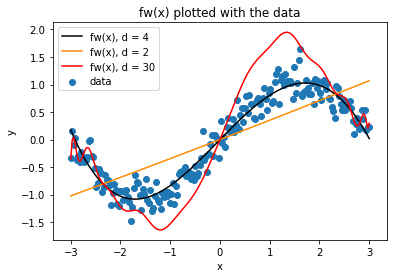
\includegraphics[width=0.5\linewidth]{fwx}
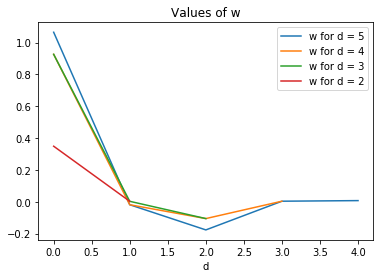
\includegraphics[width=0.5\linewidth]{calcw}
The most crucial parts of the code can be seen below. $fw$ calculates the y-value of the function at the given points in the xvector. $calcw$ calculates each of the values of the vector $w$ with a given dimension $d$:
\begin{verbatim}
def fw(w,x):
    retVal = 0
    for j in range(len(w)):
        retVal = retVal + w[j]*(x**(j+1))
    return retVal
    
def calcW(d, matrix):
    yVec = matrix[:,1].copy()
    xVec = data[:,0].copy()
    xmat = np.empty([len(matrix[:,0]), d])
    
    for i in range(len(xVec)):
        for j in range(d):
            xmat[i][j] = xVec[i]**(j+1)

    return inv(xmat.transpose() @ xmat) @ xmat.transpose() @ yVec
\end{verbatim}